%% USPSC-Introducao.tex

% ----------------------------------------------------------
% Introdução (exemplo de capítulo sem numeração, mas presente no Sumário)
% ----------------------------------------------------------
\chapter[Introduction]{Introduction}
\label{ch: Intro}

During the last decade, the world has seen an increase in participation of renewable sources in power generation, leaded mainly by wind and solar energy. These green technologies provide an alternative to sources based on fossil fuel, lowering pollution levels and reducing greenhouse gas emissions. On the other hand, the power output from these sources rely on weather conditions and can't be fully controlled.

This increase is seen worldwide, as part of policies to reduce the human impact on climate and the environment. This `renewable wave' is leaded mainly by European countries, specially in the European Union (EU), United States (US) and China. In particular, EU has set in 2010 a strategy plan to reduce its greenhouse emissions by at least 20\% compared to 1990 levels and increase the share of renewable sources to at least 20\% by 2020 \cite{Europe2020}.

Brazil does not lag far behind EU regarding renewable sources policies. In 2002, the country passed a bill that, among other actions, creates the Program of Incentive to Alternative Electric Energy Sources (PROINFA). This program aims to increase the share of wind, solar, small hydro and biomass energy production. The final goal is to have these resources corresponding to 10\% of Brazil's annual energy consumption \cite{Brazil2002}.

\section{Wind Energy}

Those policies stimulated the increase of wind energy participation, reaching a scenario where it is the main energy source of some countries. In the EU, wind energy alone generated 362 TWh in 2018, covering 14\% of the electricity demand, a share 2\% higher than 2017. Breaking down to countries, Denmark leads in this sector, with 41\% of its demand supplied by wind power plants, followed by Ireland (28\%), Portugal (24\%) and Germany (21\%). The total installed capacity across the 28 EU countries is 178.8 GW, with Germany in first position, with a total installed capacity of 59.3 GW, followed by Spain and the United Kingdom (UK), with 23.5 and 21.0 GW installed, respectively \cite{WindEurope2019}. Figure \ref{fig: EUrank} displays the detailed percentage of electricity demand covered by wind in the EU.

\begin{figure}[]
	\caption{Share of electricity demand in the EU covered by wind energy}
	\begin{center}
		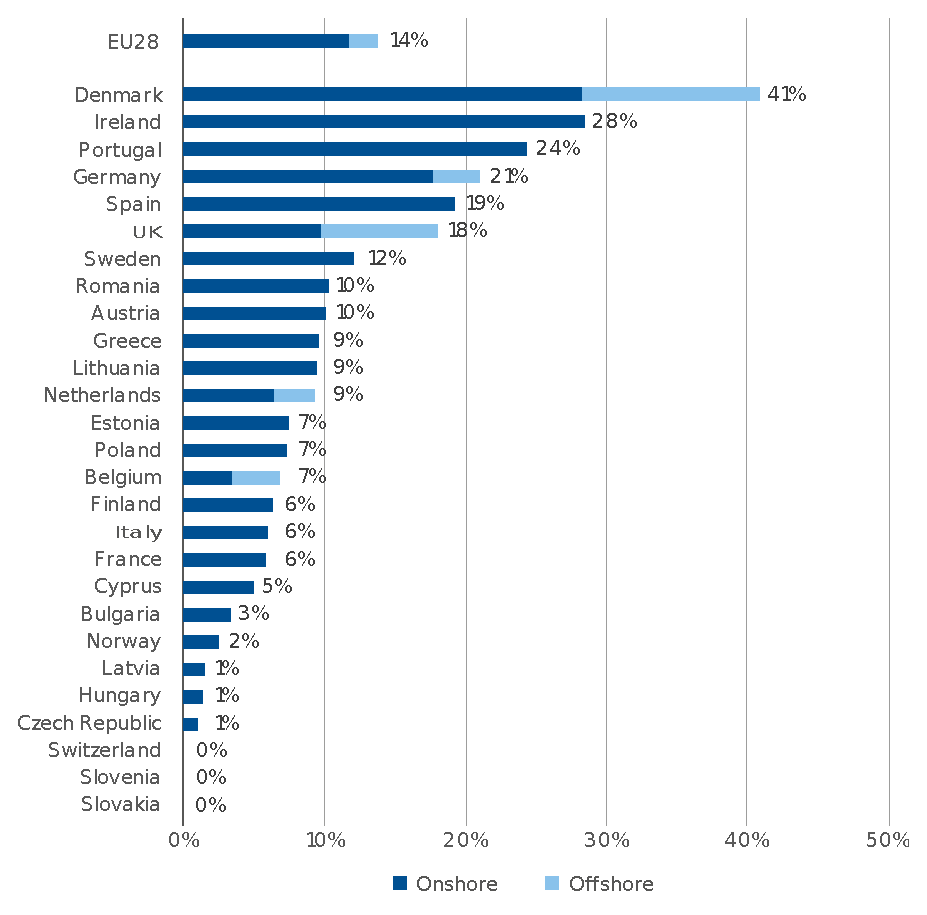
\includegraphics[scale=0.5]{Images/EUrank.eps}
	\end{center}
	\label{fig: EUrank}
	\legend{Source: Wind Europe}	
\end{figure}

In Brazil, wind energy contributed with 42.4 TWh during 2017, resulting in a participation share of 7.2\%. But, while other sources, such as hydro and coal, had its share lowered, wind energy had the highest variation among sources comparing to 2016, increasing its contribution by 26.5\% \cite{EPE2018}. In therms of installed capacity, wind power plants appear in \nth{2} place, with 14.7 GW installed, only behind hydro power plants \cite{ABEEolica2018}, as shown in Figure \ref{fig: BRshare}.

\begin{figure}[b]
	\caption{Electricity generation in Brazil by source}
	\begin{center}
		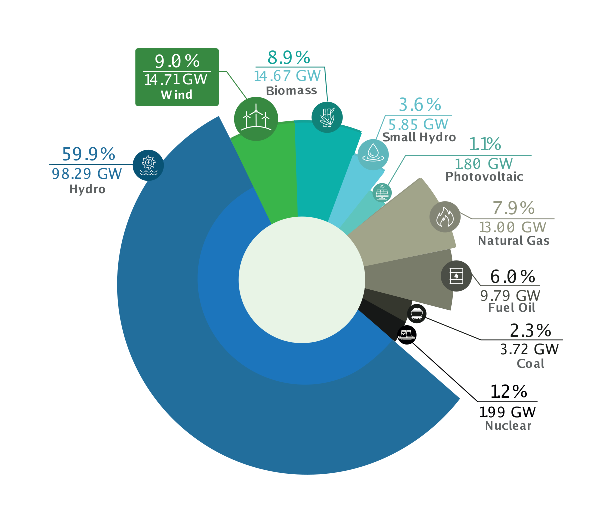
\includegraphics[scale=0.75]{Images/BRshare19.eps}
	\end{center}
	\label{fig: BRshare}
	\legend{Source: ABEE\'olica}
\end{figure}

However, there is plenty of energy yield for this source to be explored. Studies show that Brazil has potential to generate 272.2 TWh per year, with an installed capacity of 143.5 GW. The Northeast Region has the higher potential, with an annual energy yield of 144.3 TWh and potential to host up to 75.0 GW \cite{Atlas2001}. Also, the wind regime in the Northeast Region is complimentary to the water regime of the main river responsible to power generation in the region, as presented by Figure \ref{fig: WindWater}. This characteristic would help controlling reservoir water level during dry season, an important resource not only for power generation, but also irrigation of crops and water supply \cite{ANEEL2005}.

\begin{figure}
	\caption{Wind and water regime in the Northeast Region}
	\begin{center}
		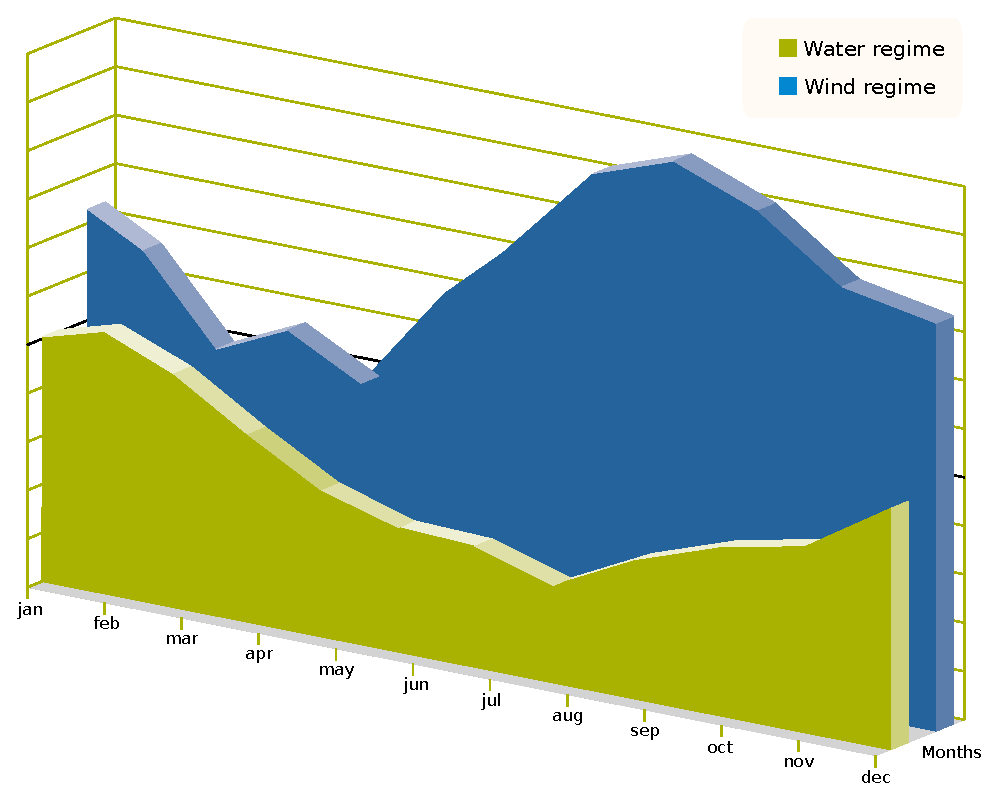
\includegraphics[scale=0.5]{Images/WindWater.eps}
	\end{center}
	\label{fig: WindWater}
	\legend{Source: ANEEL}
\end{figure}

With all this information in hand, it is only reasonable to assume that wind energy will increase its participation in electricity generation. But, in order to allow this growth, studies about how wind generators and power plants behave during faults in the grid are needed.

\section{Wind Turbine Model}

With a growing share of energy covered by wind, system operators must consider how wind turbines affect the system stability during faults and maneuvers. To do so, mathematical models capable of describing these machines' behaviour are crucial. Obtaining these models, on the other hand, is not an easy task, due to considerable amount of wind turbines in large power plants, with different manufacturers, technologies, sizes, distances from point of connection and wind conditions. Thus, a model that describes well a particular turbine in a power plant, won't necessarily work for its neighboring generators. Also, due to industrial secrecy, manufacturers provide little or no information about how their turbines behave. Furthermore, having one model for every wind turbine within a power plant would result in a mathematical problem with high complexity and computational cost \cite{Erlich2012}.

To address this problem, studies such as \cite{Muljadi2008}, \cite{Ellis2011}, \cite{council2008wecc} and \cite{Asmine2011}, motivated specially by the Institute of Electrical and Electronics Engineers (IEEE) and the Western Electricity Coordinating Council (WECC), developed generic models able to predict the behaviour of entire wind power plants. Such models reduced the problem complexity, since they were composed of a single equivalent generator. A two-machine model is needed only in rare cases, such as when the wind power plant is composed of two or more types of wind turbines \cite{Ellis2011}.

These studies have also shown that commercial wind turbine generators could be sorted into four basic types, according to its technology \cite{Ellis2011}. These types are described in the following subsections.

\subsection{Type-1 Wind Turbine Generator}

The first type of wind turbine generator is composed of a Squirrel Cage Induction Generator (SCIG) connected to a wind turbine through a controlled gearbox, as displayed in Figure \ref{fig: WTG1}. Due to its torque-speed characteristics, generators of this type operate at constant rotor speed, requiring robust controllers on gearbox and blade. Besides, as usual to any induction generator, the SCIG absorbs reactive power during operation. Thus, capacitors are often employed for power faction correction purposes. Moreover, type-1 generators limit aerodynamic power by varying the pitch angle of their blades, imposing great mechanical stress on blades, shafts and gears, demanding a robust mechanical design and preventing these generators to operate above certain wind speed \cite{Ellis2011}. 

\begin{figure}[h]
	\caption{Representation of Type-1 Wind Turbine Generator}
	\begin{center}
		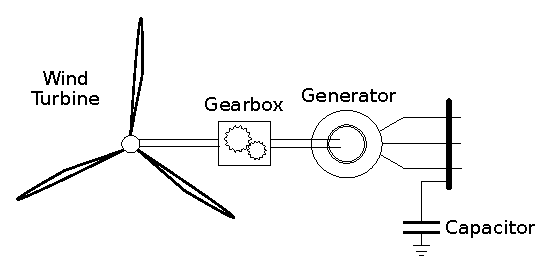
\includegraphics[scale=1]{Images/Type1WTG.eps}
	\end{center}
	\label{fig: WTG1}
\end{figure}

\subsection{Type-2 Wind Turbine Generator}

Similarly to Type-1 Wind Turbine Generator, Type-2 generators are composed of an asynchronous machine connected to a wind turbine via gearbox, but, instead of SCIG, Wound Rotor Induction Generator (WRIG) are used to convert kinetic energy into electricity. The WRIG has access to its rotor windings, allowing to vary the rotor resistance. As a direct consequence, this machine can operate in different wind speeds by adjusting its torque-speed curve as needed \cite{Ellis2011}. Therefore, Type-2 Wind Turbine Generators have a WRIG with a variable resistance connected to its rotor terminals, as shown in Figure \ref{fig: WTG2}.

\begin{figure}[h]
	\caption{Representation of Type-2 Wind Turbine Generator}
	\begin{center}
		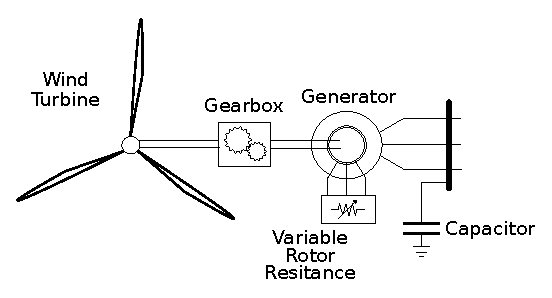
\includegraphics[scale=1]{Images/Type2WTG.eps}
	\end{center}
	\label{fig: WTG2}
\end{figure}

This type of generator has then three speed control systems, with rotor resistance control responding to rapid changes in speed, gearbox control for medium variations and pitch control for slow changes. These control system work together to maintain power output constant and reduce mechanical stress on components. The effects on the torque-speed curve caused by different rotor resistances are shown in Figure \ref{fig: Tw}. For a fixed power, increasing rotor resistance increases the speed needed on the shaft, allowing the wind turbine to operate above rated wind speed. However, the speed range is only $\pm 10\%$ of rated slip. Also, this machine still needs a reactive compensation circuit on its terminals \cite{Muljadi2010}.

\begin{figure}[h]
	\caption{Torque-speed curve}
	\begin{center}
		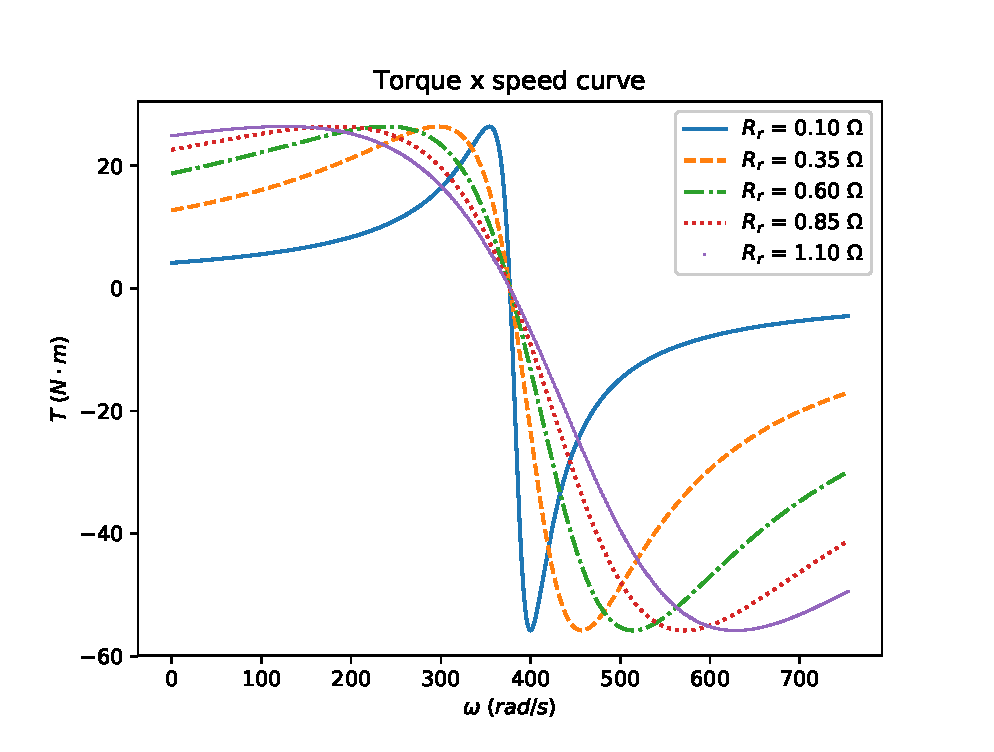
\includegraphics[scale=.7]{Images/Tw_curve.eps}
	\end{center}
	\label{fig: Tw}
\end{figure}

\subsection{Type-3 Wind Turbine Generator}

A Type-3 Wind Turbine Generator, often called Doubly Fed Induction Generator (DFIG), is also composed of a wound rotor machine connected to a wind turbine. But, instead of varying rotor resistance, a DFIG has its rotor supplied with AC voltage by a back-to-back frequency converter, as displayed in Figure \ref{fig: WTG3}. By varying the voltage frequency on the rotor circuit, the generator is able to supply power to the grid in a wider range of wind speed, reaching up to $\pm 30\%$ of rated slip. In addition, the converter can control both real and reactive power independently, ending the necessity of capacitors \cite{Muljadi2010}. Since approximately 30\% of rated power flows through the rotor windings, power electronics components have lower specifications and don't have great impact on overall costs. On the other hand, these generators need regular maintenance due to slip rings, brushes and gearbox, preventing its use in offshore applications \cite{Yaramasu2015}.

\begin{figure}[h]
	\caption{Representation of Type-3 Wind Turbine Generator}
	\begin{center}
		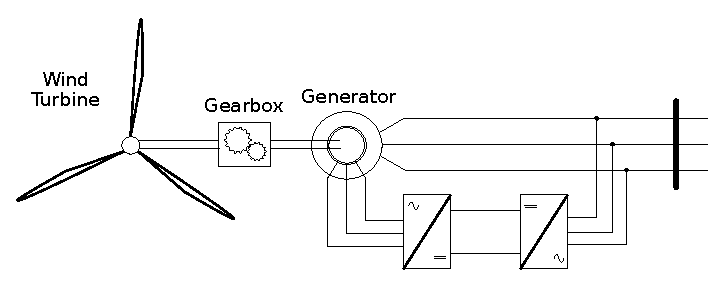
\includegraphics[scale=1]{Images/Type3WTG.eps}
	\end{center}
	\label{fig: WTG3}
\end{figure}

\subsection{Type-4 Wind Turbine Generator}

The last type of wind turbine generator, also called Full-Converter Generator, is composed of a electrical machine connected to the grid through a back-to-back frequency converter. The converter will operate converting the electrical frequency generated to standard, allowing this type of wind turbine generator to operate in a large range of wind speed (up to almost 100\% of rated slip). Due to the converter operation, connection to the wind turbine can be made directly or via gearbox. Likewise, it allows the use of synchronous and asynchronous electrical machines as generator, with Permanent Magnet Synchronous Generator (PMSG), Electrical Excited Synchronous Generator (EESG) and SCIG being most common, because of cost and maintenance purposes. Similar to DFIG, full-converter generators are able to control real and reactive power injected into the grid. However, since all power generated must flow through the power electronics, the overall cost of these generators is usually higher \cite{Yaramasu2015}. Figure \ref{fig: WTG4} depicts a typical Type-4 Wind Turbine Generator.

\begin{figure}[h]
	\caption{Representation of Type-4 Wind Turbine Generator}
	\begin{center}
		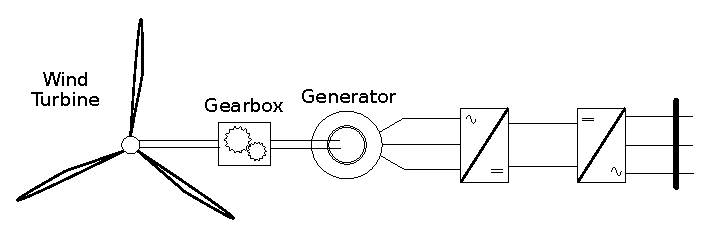
\includegraphics[scale=1]{Images/Type4WTG.eps}
	\end{center}
	\label{fig: WTG4}
\end{figure}

Figure \ref{fig: WindShare} shows the evolution of share in installed capacity onshore for each generator type. The data shows how SCIG and WRIG lost space in the segment and how DFIG and Full-Converter Generators' participation rose, dominating the global market \cite{Magagna2017}.

\begin{figure}[h]
	\caption{Share of installed capacity for each wind turbine generator type}
	\begin{center}
		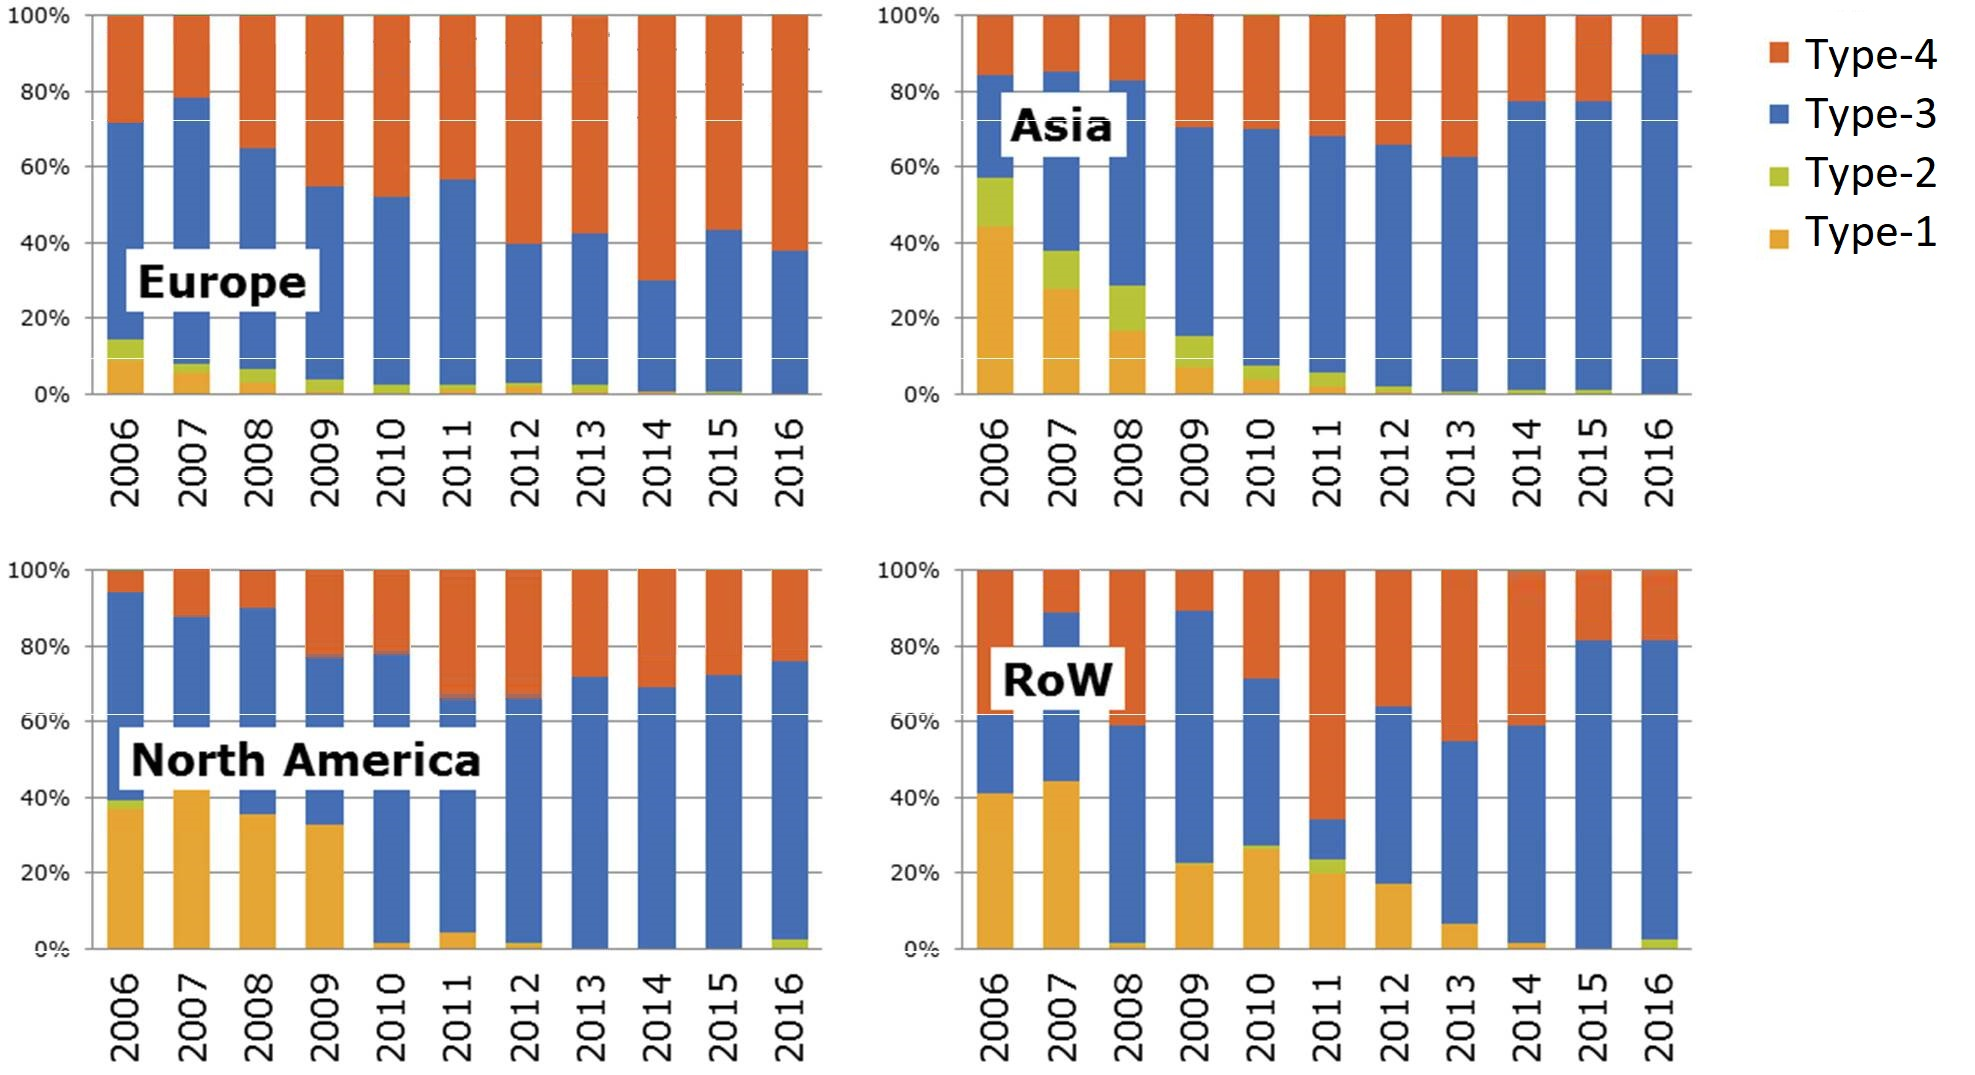
\includegraphics[scale=.2]{Images/WTGTypes.jpg}
	\end{center}
	\legend{Source: JRC}
	\label{fig: WindShare}
\end{figure}

In the light of the data presented above, this work aims to develop a software able to estimate the parameters of a mathematical model capable of predict the behaviour of Type-3 Wind Turbine Generators. The DFIG mathematical model will be subject to the following chapter. Afterwards, the estimation process and methods will be presented on chapter \ref{ch: Est}. At last, partial results and future prospects will be presented on chapter \ref{ch: Res}.
